\documentclass[12pt,aspectratio=169]{beamer}

\usetheme[progressbar=frametitle, numbering=fraction]{metropolis}
\usepackage{appendixnumberbeamer}
\usepackage{gensymb}
\usepackage{booktabs}
\usepackage[scale=2]{ccicons}

\usepackage{pgfplots}
\usepgfplotslibrary{dateplot}
\usepackage[english]{babel}

\usepackage{xspace}
\newcommand{\themename}{\textbf{\textsc{metropolis}}\xspace}

\usepackage{amsmath}

% Chinese Fonts (Fontset: fandol,ubuntu)
\usepackage[fontset=fandol]{ctex}

% Math Fonts
\usefonttheme{professionalfonts}
\usepackage{mathspec}
\setsansfont[BoldFont={Fira Sans},
  Numbers={OldStyle}]{Fira Sans Light}
\setmathsfont(Digits)[Numbers={Lining, Proportional}]{Fira Sans Light}

% Change Color of the theme
\usepackage{xcolor}
\definecolor{DarkGrey}{HTML}{353535}
\definecolor{ECNURed}{RGB}{164,31,53}
\definecolor{ECNUBrown}{RGB}{134,117,77}
\definecolor{BackGround}{RGB}{250,250,250}
\definecolor{MyBlue}{RGB}{0,161,233}
\definecolor{MyRed}{RGB}{228,0,127}
\setbeamercolor{normal text}{ fg= DarkGrey  }
\setbeamercolor{alerted text}{ fg= ECNURed  }
\setbeamercolor{example text}{ fg= ECNUBrown  }

% Bolder Fonts for presenting in a large room 
\setsansfont[BoldFont={Fira Sans SemiBold}]{Fira Sans}
\metroset{block=fill}

\usepackage{listings,xcolor}
\usepackage{tikz}
\usepackage{pgfmath}
\usepackage{animate,media9,graphicx}
\usepackage{calligra}
\usepackage{array}
\renewcommand{\arraystretch}{2}  % 增加行高
\setlength{\tabcolsep}{10pt}     % 增加列间距

\lstset{
  language         = c++,
  numbers          = left,
  numberstyle      = \tiny,
  breaklines       = true,
  captionpos       = b,
  tabsize          = 4,
  frame            = shadowbox,
  columns          = fullflexible,
  commentstyle     = \color[RGB]{0,128,0},
  keywordstyle     = \color[RGB]{0,0,255},
  basicstyle       = \tiny\ttfamily,
  stringstyle      = \color[RGB]{148,0,209}\ttfamily,
  rulesepcolor     = \color{red!20!green!20!blue!20},
  showstringspaces = false,
}

\title{Machine Learning for Weather and Climate}
\subtitle{}
\author{Yifei Ding}
\date{\today}
% \institute{演讲者描述}
% \titlegraphic{\hfill
\includegraphics[height=1.5cm]{ECNUlogo.png}}

\begin{document}

\maketitle
% \footnotesize
% \begin{frame}{Contents}
%   \setbeamertemplate{section in toc}[sections numbered]
%   \tableofcontents%[hideallsubsections]
% \end{frame}

\begin{frame}{Background and Preliminaries}
  \begin{block}{Weather Forecasting}
    Given a dataset ${\cal D}=\{X_i\}_{i=1}^N$ of history weather data, forecast future weather conditions
    $X_T\in\mathbb{R}^{V\times H\times W}$ with initial conditions $X_0\in\mathbb{R}^{V\times H\times W}$.

    $T$: target lead time, $V$: number of input and output variables, $H\times W$: spatial resolution.
  \end{block}

  Three major approches: 
  \begin{itemize}
    \item \textit{\color{ECNURed}direct forecasting}
    \item \textit{\color{ECNURed}continuous forecasting}
    \item \textit{\color{ECNURed}iterative forecasting}
  \end{itemize}
\end{frame}

\begin{frame}{ClimaX}
  Object: design and train a foundation and efficient model for weather and climate concerning atmosphere.

  Model architecture:
  \begin{itemize}
    \item \textit{\color{ECNURed}Variable tokenization}: tokenize the input into 
    $V\times (H/p)\times (w/p)=\allowbreak V\times h\times w$ 
    patches, and embed each input patch os size $p^2$ to a vector of dimension $D$;

    \item \textit{\color{ECNURed}Variable aggregation}: perform a cross-attention operation for each spatial position in the 
    $h\times w$ map;

    \item \textit{\color{ECNURed}Transformer}: extend a standard ViT to generate the output tokens.
  \end{itemize}
\end{frame}

\begin{frame}{ClimaX}
  \begin{figure}
    \begin{center}
      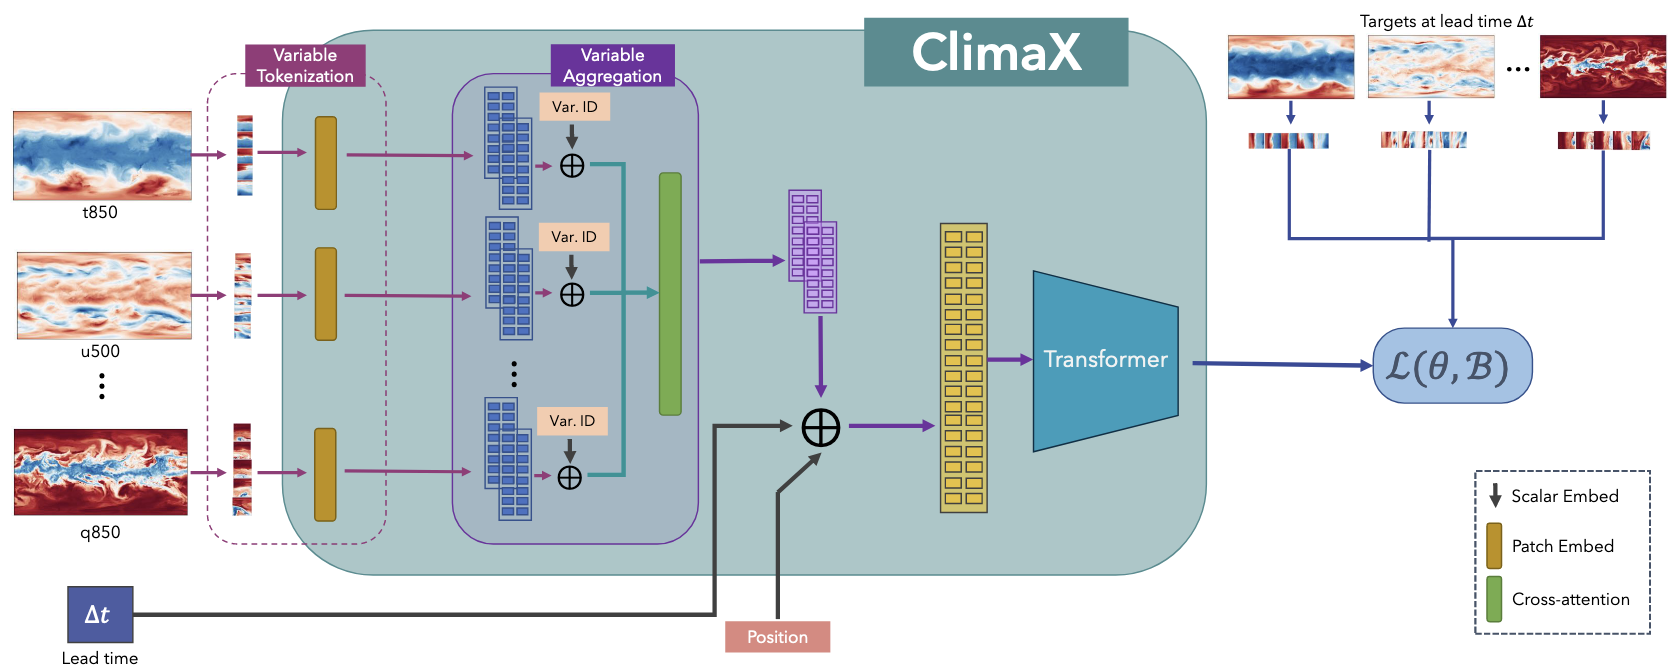
\includegraphics[width=0.85\textwidth]{figures/ClimaX.png}
    \end{center}
    \caption{Pretraining phase of ClimaX}\label{fig:1}
  \end{figure}
\end{frame}

\begin{frame}{Stormer}
  A simple, skillful and competitive model for weather forecasting.

  Training: \textit{\color{ECNURed}randomized dynamics forecasting objective}
  $$
    {\cal L}(\theta)=\mathbb{E}_{\delta t\sim P(\delta t),(X_0,X_{\delta t})\sim {\cal D}}
    \left[||f_{\theta}(X_0,\delta t)-\Delta_{\delta t}||_2^2\right]
  $$

  With pressure-weighted loss and multi-step finetuning, the final loss function is
  $$
    {\cal L}(\theta)=\mathbb{E}\left[\frac{1}{KVHW}\sum_{k=1}^K\sum_{v=1}^V
    \sum_{i=1}^H\sum_{j=1}^Ww(v)L(i)(\hat\Delta_{k\delta t}^{vij}-\Delta_{k\delta t}^{vij})^2\right].
  $$
\end{frame}

\begin{frame}{Stormer}
  Inference: use two inference strategies, \textit{\color{ECNURed}homogeneous} and 
  \textit{\color{ECNURed}best m in n}, and obtain the final prediction by averaging the individual predictions.

  Model architecture: 
  \begin{itemize}
    \item apply \textit{\color{ECNURed}ViT} for this task.

    \item Weather-specific embedding: \textit{\color{ECNURed}variable tokenization} and 
    \textit{\color{ECNURed}variable aggregation}.

    \item Stormer Transformer block: replace standard layer normalization with \textit{\color{ECNURed}adaLN} 
    and regress parameters with an \textit{\color{ECNURed}one-layer MLP} from the embedding of $\delta t$.
  \end{itemize}
\end{frame}

\begin{frame}{ClimateLearn}
  Propose a PyTorch library implementing a range of functionalities for benchmarking of ML models for
  weather and climate.
  \begin{itemize}
    \item Tasks: weather forecasting, downscaling, climate projection.
    \item Datasets: ERA5, Extreme-ERA5, CMIP6, PRISM.
    \item Models: traditional baselines, deep learning models.
    \item Evaluations: forecasting metrics, downscaling metrics, climate projection metrics, visualization.
  \end{itemize}
\end{frame}

\begin{frame}{Acknowledgement}
  \begin{center}
    \textcolor{gray}{\Huge{\centerline{\calligra{Thank you!}}}}
  \end{center}
\end{frame}

\end{document}
